\scanpage{21}
\diagram{\begin{tikzcd}[ampersand replacement=\&,column sep=small,row sep=small]A\arrow[dr,dash]\&\&B\arrow[dl,dash]\\\&S\&\end{tikzcd}}
\margin{schémas abéliens sur $S$}
\[
u_p:T_p(A)\mathbin{-}T_p(B)
\]
Question: quand \unsure{ceci} provient-il d'un hom $u:A\mathbin{-}B$.
\deleted{(i) À cause de l'unicité, \unsure{la desc est fid. plate universelle}}
\deleted{(ii) l'ens \inserted{$T$} des pts $s\in S$ tels que $u_{ps}:T_p(A_s)\mathbin{-}T_p(B_s)$ provienne de $u_s:A_s\longrightarrow B_s$ (condition géom. par (i)) est \uline{fermé}.
\deleted{Si $t\in T$ est tel que car. $k(t)=$}
(iii) Si $t\in T$ est tel que car $k(t)=p$, alors $\exists$ voisinage ouvert $U$ de $t$ tel que $u_p|U$ soit algébrique, en particulier \unsure{$t$ est un pt intérieur de $T$}.}

\figure{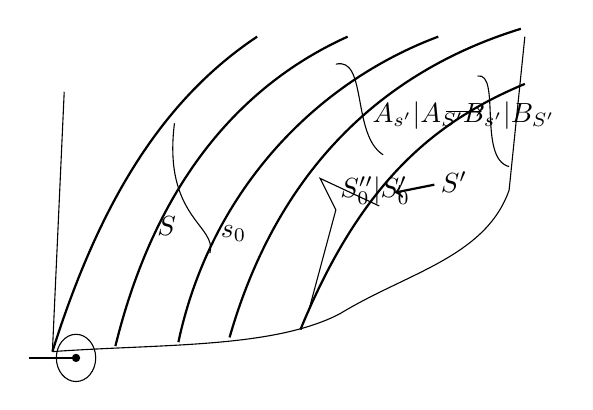
\begin{tikzpicture}[x=1cm,y=1cm]
\draw (0,0)--(.15,3.3);\draw (0,0) .. controls (1.4,.1) and (2.8,.04) .. (3.65,.48) .. controls (4.5,1.0) and (5.5,1.2) .. (5.8,2.05)--(6,4.0);
\draw[line width=.8pt] (0,0) .. controls (.6,1.9) and (1.4,3.2) .. (2.6,4.0);
\draw[line width=.8pt] (.8,.07) .. controls (1.25,1.9) and (2.2,3.3) .. (3.75,4.0);
\draw[line width=.8pt] (1.6,.12) .. controls (2,2.0) and (3.3,3.4) .. (4.9,4.0);
\draw[line width=.8pt] (2.25,.18) .. controls (2.8,2.1) and (4,3.5) .. (5.95,4.1);
\draw[line width=.8pt] (3.15,.28) .. controls (3.9,2.1) and (4.8,2.9) .. (6,3.4);
\draw (1.55,2.9) .. controls (1.4,1.7) and (2.1,1.6) .. (2.0,1.25);\node at (1.45,1.6){$S$};\node at (2.3,1.5){\deleted{$\unsure{s_0}$}};
\draw (3.25,.5)--(3.6,1.8)--(3.4,2.2)--(4.15,1.85);\node at (4.1,2.05){$\unsure{S''_0|S'_0}$};\node at (5.1,2.15){$S'$};\draw[->,thick](4.85,2.12)--(4.35,2.02);
\draw (3.6,3.65) .. controls (4,3.75) and (3.8,2.75) .. (4.2,2.5);\draw (5.4,3.5) .. controls (5.7,3.55) and (5.4,2.45) .. (5.8,2.35);
\node at (4.65,3.0){$\unsure{A_{s'}|A_{S'}}$};\node at (5.8,3.0){$\unsure{B_{s'}|B_{S'}}$};\draw[->](5.0,3.05)--(5.45,3.05);
\fill (.3,-.08) circle (1.5pt);\draw (.3,-.08) ellipse (.25 and .3);\draw[thick](-.3,-.08)--(.3,-.08);
\end{tikzpicture}}

a) Il y a \inserted{(si $S$ noeth)} un plus grand sous-schéma $\unsure{\overline S|T}$ de $S$ sur lequel $u_p$ est algébrique; $T$ est fermé, sa \unsure{formati-} commute à tout changt de base (nouvelles bases pas \unsure{néc.} noethériennes).

b) Si $t\in T$ est tel que car $k(t)=p$, alors $T$ contient un voisinage ouvert induit de $t$. \deleted{Donc si $S_p=V(p1_S)$, alors $T$ est un voisinage (\unsure{ouvert-et-fermé}) de $T\cap S_p$}

\deleted{\uline{Cor.} Supposons que pour tout $s\in\operatorname{Ass}O_S$,}
\deleted{\uline{Corollaire} Supposons que pour tout $s\in$}

\uline{Cor.} Soit $Z$ l'ens \deleted{des éléments de $\operatorname{Max}S$ \unsure{et de} (pts maximaux de $S$) et de l'ens des} \inserted{des pts de $S$ qui sont} maximaux, ou qui sont associés \deleted{\unsure{et}} à $O_S$ \uline{et} de car. $\ne p$. Supposons que $z\in Z\Longrightarrow\exists s\in\overline{\{z\}}$ tel que $k(s)$ de car. $p$ et $s\in T$ \inserted{(i.e. $\overline{\{z\}}\cap S_p\cap T\ne\varnothing$)}. Alors $u_p$ est algébrique.
\mspage{20}
